\documentclass[tikz,border=2pt]{standalone}
\usepackage{amsmath}
\usepackage{pgfplots}
\pgfplotsset{compat=1.18}

\begin{document}
% Power functions x^k for several exponents: an even power, an odd power, a root and a negative
% power. The exponent decides the shape, the symmetry and the natural domain.
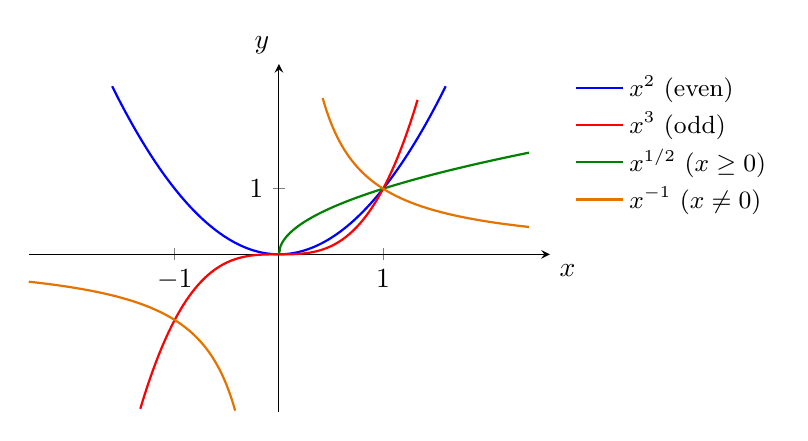
\begin{tikzpicture}
	\begin{axis}[
		axis lines=middle,
		xmin=-2.4, xmax=2.6,
		ymin=-2.4, ymax=2.9,
		xtick={-1,1}, ytick={1},
		xlabel={$x$}, ylabel={$y$},
		xlabel style={below right}, ylabel style={above left},
		samples=160, smooth, clip=false,
		width=8.2cm, height=6cm,
		legend pos=outer north east, legend style={draw=none, fill=none, font=\small}, legend cell align=left
		]
		\addplot[thick, blue, domain=-1.6:1.6] {x^2};
		\addlegendentry{$x^2$ (even)}
		\addplot[thick, red, domain=-1.33:1.33] {x^3};
		\addlegendentry{$x^3$ (odd)}
		\addplot[thick, green!50!black, domain=0:2.4] {sqrt(x)};
		\addlegendentry{$x^{1/2}$ ($x\ge0$)}
		\addplot[thick, orange!90!black, domain=0.42:2.4] {1/x};
		\addplot[thick, orange!90!black, domain=-2.4:-0.42] {1/x};
		\addlegendentry{$x^{-1}$ ($x\neq0$)}
	\end{axis}
\end{tikzpicture}
\end{document}
